\section[Промышленная СППР Analytica]
{ПРОМЫШЛЕННАЯ СППР ANALYTICA}

\subsection{Описание рассматриваемой СППР}

Система поддержки принятия решений Analytica разработана компанией Lumina Decision Systems.
Данная система ориентирована на модели, которые представляют собой некоторый
материальный или мысленно представляемый объект или явление, замещающий
оригинальный объект или явление, сохраняя только некоторые важные его свойства,
например, в процессе познания или конструирования.

Данную СППР можно определить как программное обеспечение количественного моделирования,
как использование графического интерфейса для разработки модели.
Возможности рассматриваемой системы включают:
\begin{itemize}
  \item анализ сценариев;
  \item диаграммы влияния;
  \item многомерное моделирование (dimensional Modeling);
  \item анализ рисков.
\end{itemize}

Система обеспечивает прозрачность и мощность бизнес-моделированию. Она значительно
превышает возможности, которые предоставляются пользователям обычными электронными
таблицами, фактически это графически-ориентированное инструментальное средство
для создания, анализа и объединения количественных бизнес-моделей. Это достигается
за счёт следующих факторов:

\begin{itemize}
  \item использованию удобного графического интерфейса на основе диаграмм влияния
    для объединения моделей в общей структуре;
  \item средствам масштабирования модели, чтобы справиться с многомерностью проблем
    реального мира, используя массивы бизнес-информации (Intelligent Arrays);
  \item управлению риском и неопределенностью благодаря эффективному моделированию
    по методу Монте-Карло, который можно определить как метод моделирования
    случайных величин с целью вычисления характеристик их распределений;
  \item быстрого и легкого развертывания, создания моделей в Интернете с помощью
    инструментального средства Analytica Decision Engine®;
  \item импорта и экспорта данных с использованием механизма OLE (или
    ODBC в версии для корпорацый – Enterprise Analytica).
\end{itemize}

Из-за того, что Analytica использует графический интерфейс и малое
количество стандартных диаграммных символов, ее легко изучать и использовать.
Главный менеджер или группа менеджеров могут определить концепцию проблемы,
а её качественные аспекты могут быть отображены без применения формул.
Модели Analytica можно также легко и быстро модернизировать, поддерживать и расширять.
Массивы бизнес-информации делают возможным установление временной последовательности
моделей, исходя из того, что время является измерением. В святи с тем,
что диаграммы Analytica самодокументируются, модели легко проверять или контролировать.


\subsection{Диапазон применения СППР Analytica}

Система Analytica широко используется для создания и исследования моделей
в различных отраслях, включая: бизнес и финансы; аэропространство; консалтинг;
электронную коммерцию; здравоохранение; энергетику и окружающую среду;
разработку новых видов продукции; оборона; научно-технические исследования
и разработки, производство; телекоммуникации; высшее образование и др.

Предполагается, что пользователи системы Analytica должны быть информационно
и компьютерно грамотными, то есть понимать сущность используемой информации.
Однако компьютерная грамотность создателя решений не является обязательным
условием успешного применения СППР. Дело в том, что многие руководители
различного уровня не нуждаются в работе за компьютером, а предпочитают
ее общению с людьми. Поэтому системы поддержки принятия решений проектируются
с учетом этого фактора.

Пользователями СППР Analytica является более 25 крупных корпораций,
в частности Boeing, General Motors, Motorola, Microsoft, Xerox и др.
Среди консалтинговых пользователей системы можно назвать Anderson Consulting,
Booz-Allen \& Hamilton, Deloitte \& Touche, Ernst \& Young,
McKinsey \& Co, PriceWaterhouseCoopers, Strategic Decisions Group, SAIC.
Среди академических вузов, использующих эту систему, есть такие
ведущие университеты США и Англии, как UC Berkeley, Cambridge, Carnegie-Mellon,
Harvard, Stanford.

Analytica помогает решать сложные проблемы во многих функциональных областях,
включая: оценку проектов; финансовое моделирование; поддержку и анализ решений,
анализ, управление и ослабление риска; прогнозирование; анализ рынка;
вероятностную имитацию; сценарии \textit{<<а что ..., если ...?>>};
анализ \textit{<<затраты / выгоды>>}; экономический анализ и др.


\subsection{Способы моделирования в СППР Analytica}

Основные предоставляемые функции Analytica обеспечивает пользователя общими
языками моделирования, а также словарем более 150 операторов и функций,
включая: стандартные математические функции; финансовый анализ; тригонометрию;
создание и трансформацию многомерных массивов; матричные операторы;
интегральное и дифференциальное исчисление; текстовую последовательность
операторов; распределения вероятностей; статистический анализ; кривые сглаживания
и регрессию; анализ чувствительности и неопределенности; организацию сортировки
и индексирования; функции ODBC. ODBC (англ. Open Database Conectivity) --- это
программный интерфейс (API) доступа к базам данных, позволяющий единообразно
работать с разными источниками данных, абстрагируясь от особенностей взаимодействия
в каждом конкретном случае.

Рассмотрим пример анализа динамики и прогнозирования в системе Analytica.

Стоит заметить, что система постоянно проводит анализ динамики изменения
каждого из изучаемых показателей. Если динамика такова, что показатель
в ближайшем будущем может выйти за допустимый диапазон,
система уведомляет пользователя об этой проблеме.

График, иллюстрируюший возможность просмотра трендов по показателям приведен
на рисунке~\ref{fig:trends}.
\begin{figure}[h]
  \centering
  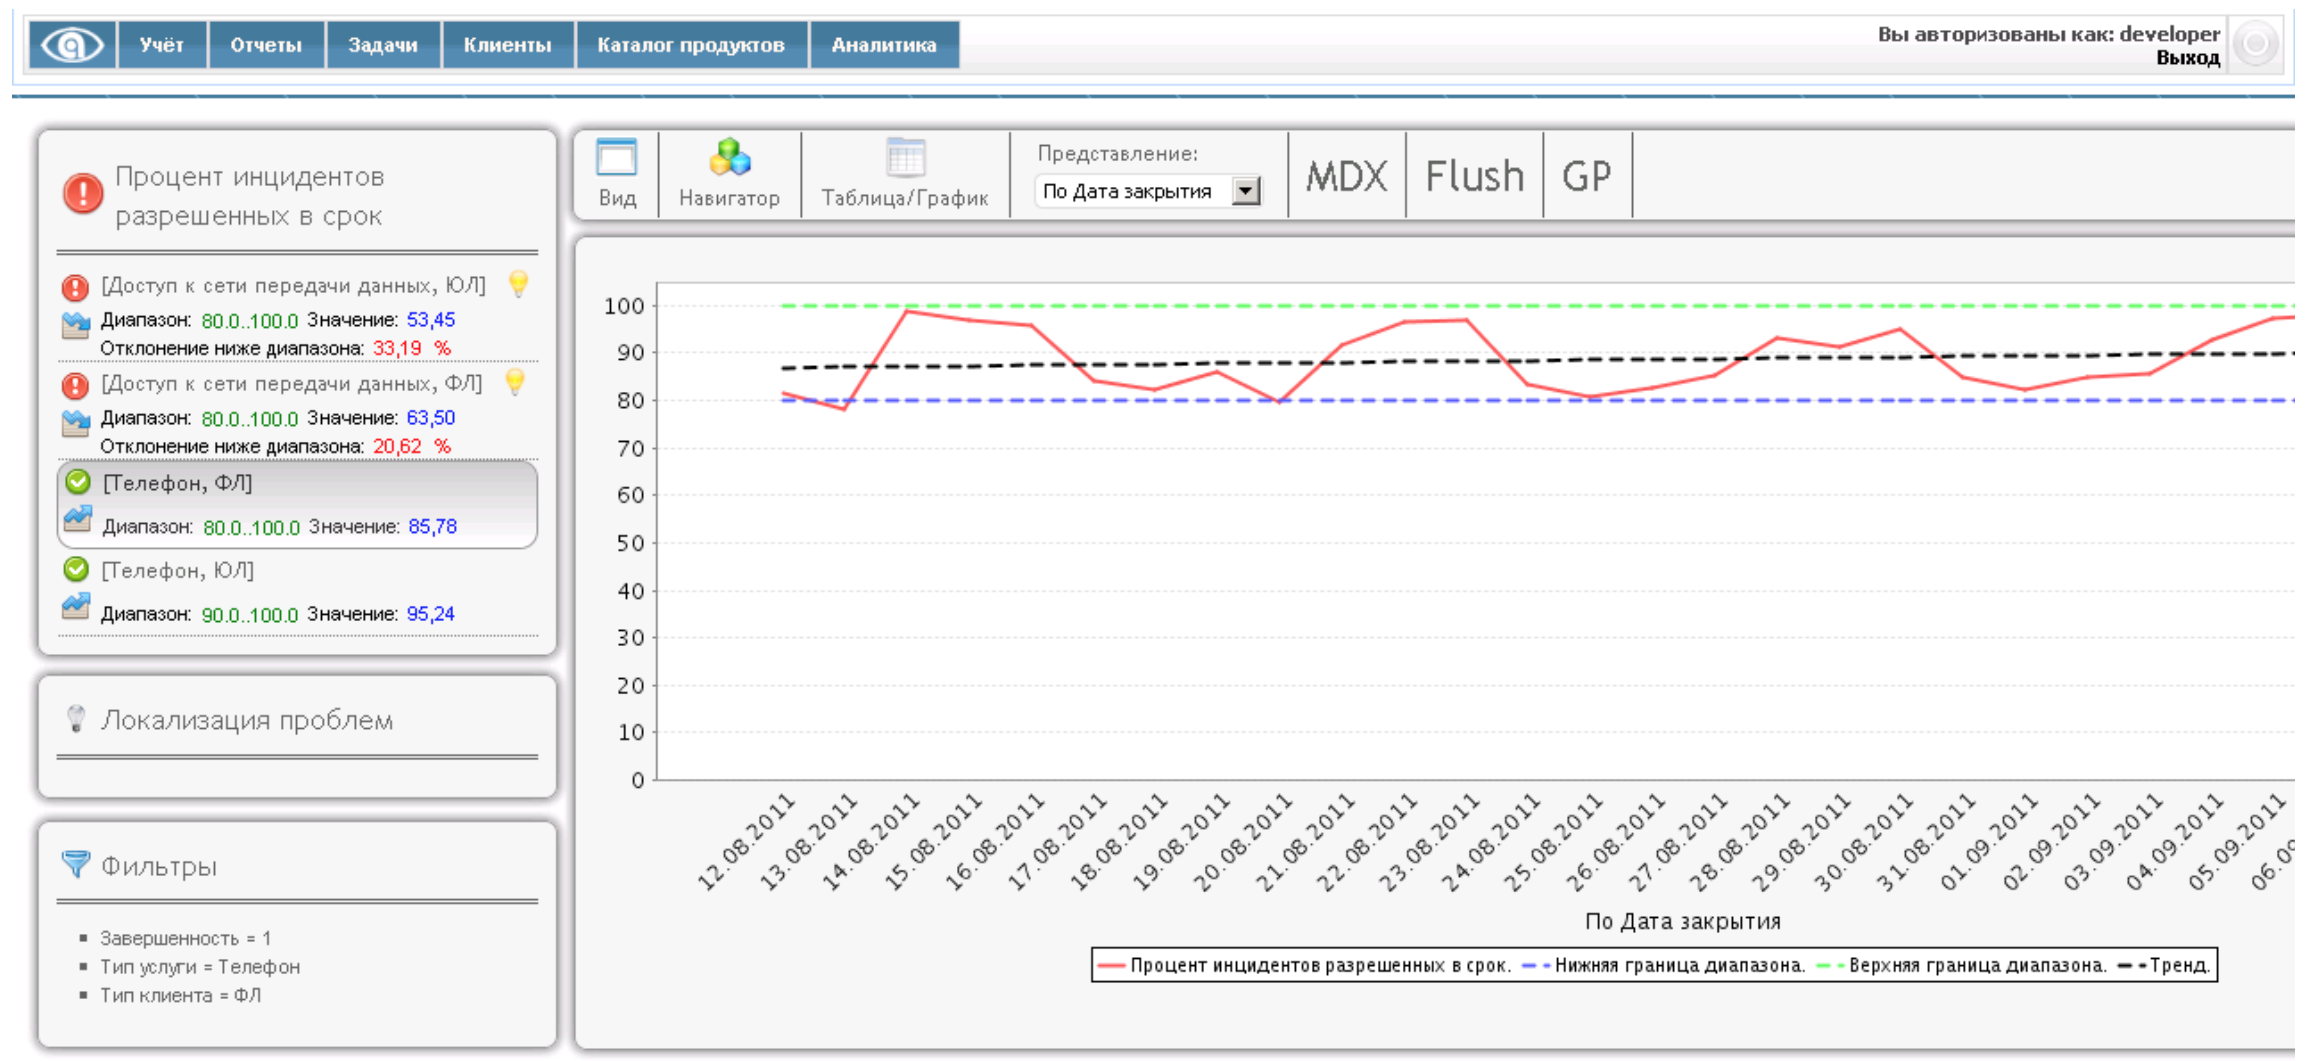
\includegraphics[scale=0.18]{fig/trends}
  \caption{Просмотр трендов по показателям в Analytica}
  \label{fig:trends}
\end{figure}

\pagebreak

Продукт Analytica помимо проведения автоматизированного анализа ориентирован
на активное взаимодействие пользователя с системой. Пользователь может делать
выборку необходимого набора данных для дальнейшего анализа. Аналитика предлагает
инструменты позволяющие облегчить создание выборки и проведение анализа:
\begin{itemize}
  \item средства многомерного анализа;
  \item фильтры;
  \item условное форматирование;
  \item возможность построения диаграмм.
\end{itemize}

Пример работы средства многомерного анализа данных приведен
на рисунке~\ref{fig:m}.
\begin{figure}[h]
  \centering
  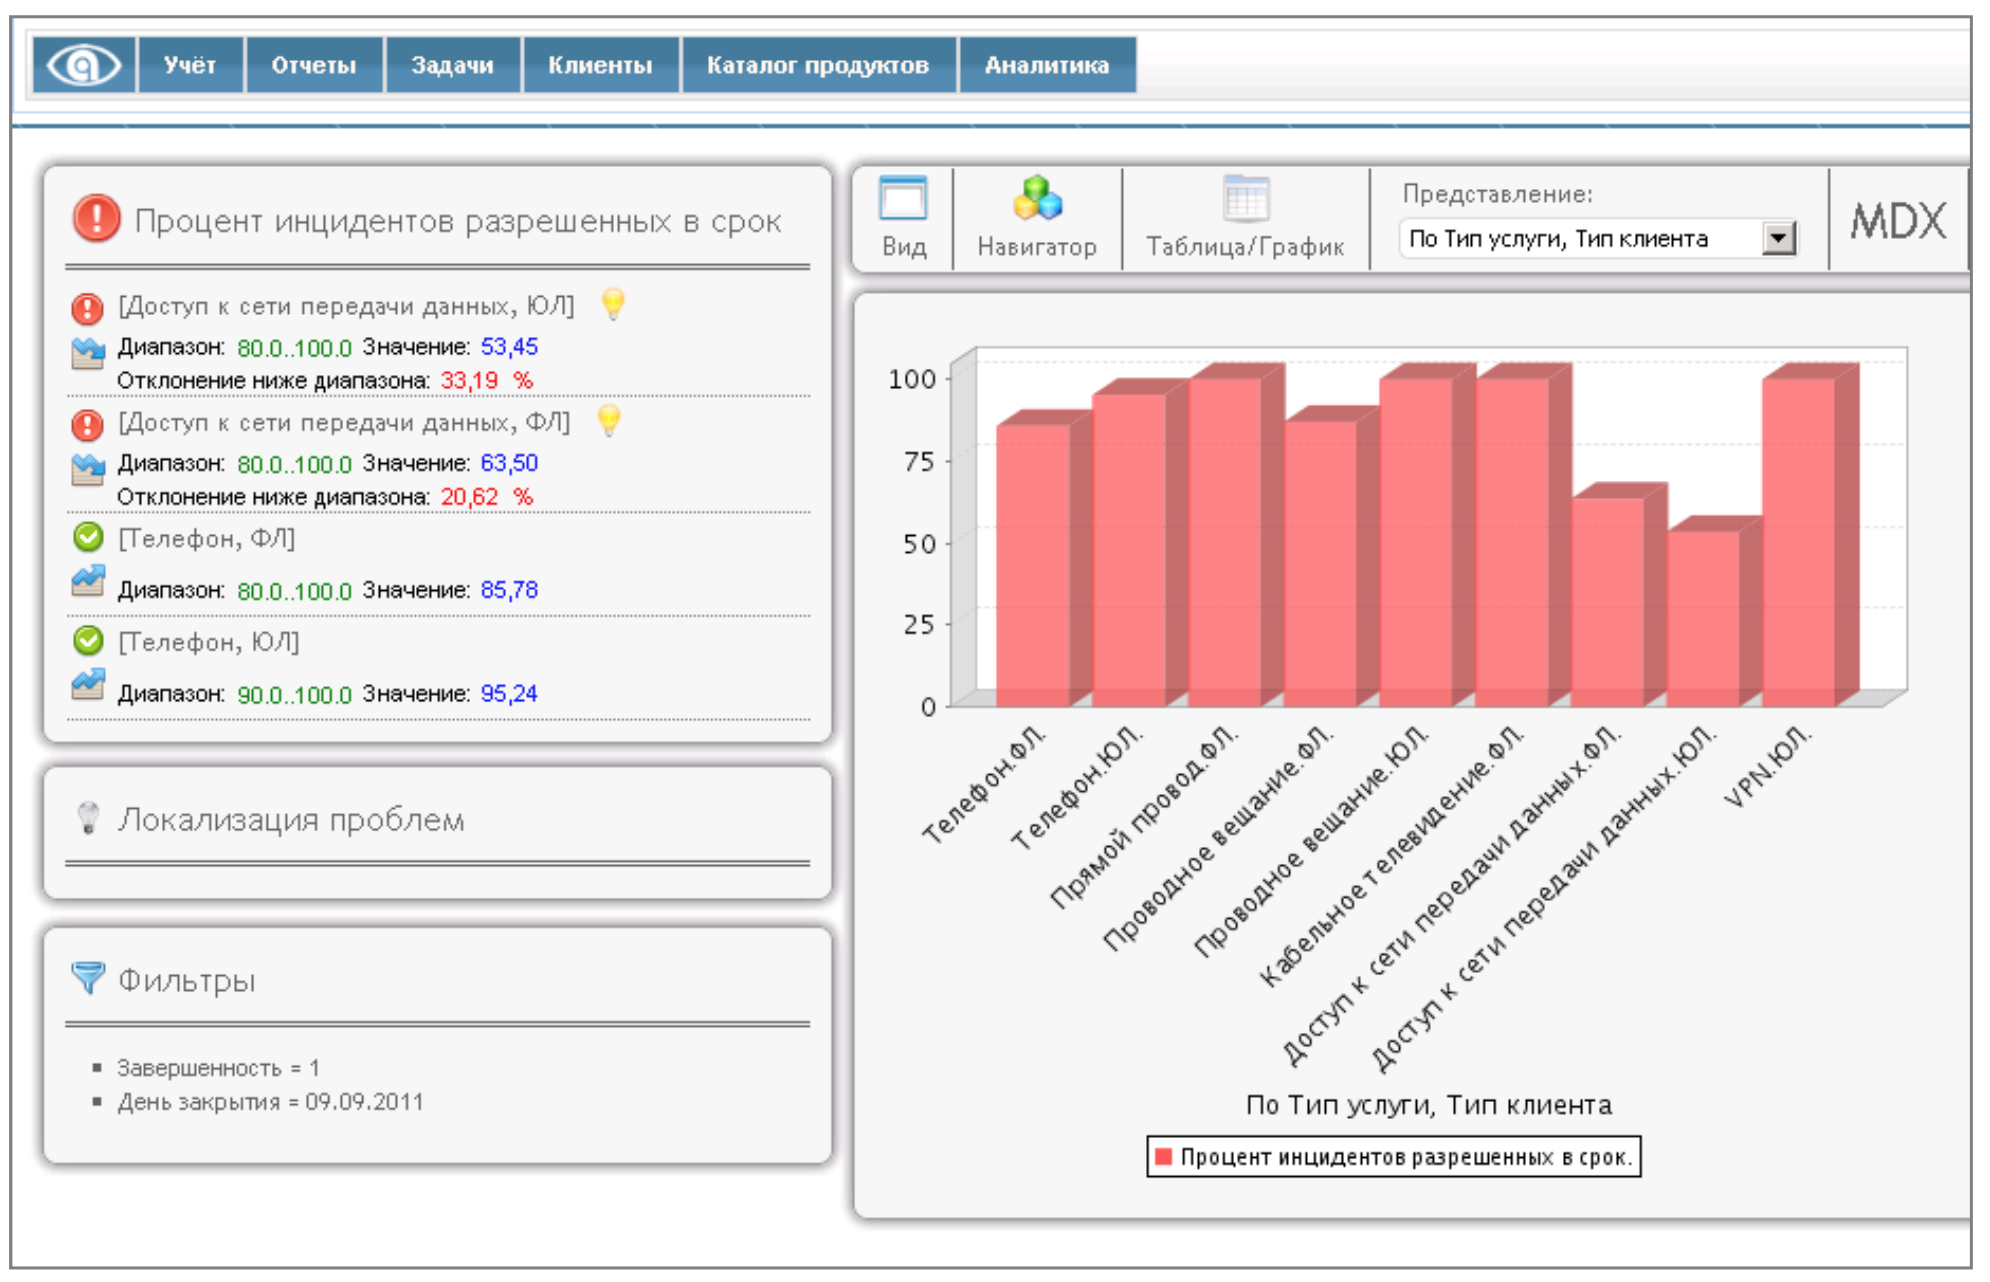
\includegraphics[scale=0.18]{fig/m}
  \caption{Просмотр многомерного анализа данных в Analytica}
  \label{fig:m}
\end{figure}

Рассмотрим подробнее процесс принятия решения и проблемы в нём. Для принятия
обоснованного решения менеджеру необходимо сначала организовать процесс
сбора необходимых данных, и затем провести их агрегацию и анализ.
В общем случае этот процесс неавтоматизирован, поэтому трудоемок, долог
и подвержен ошибкам. В общем случае этот процесс можно разбить на несколько
этопов.
\begin{enumerate}

  \item Сбор информации. Основные моменты:
    \begin{itemize}
      \item часто информация собирается из многих источников, например,
        из нескольких филиалов;
      \item не всегда у исполнителей существуют возможность и инструменты
        (отчеты информационных систем) для получения именно необходимой
        руководству информации;
    \end{itemize}

  \item Агрегация и подготовка. Основные моменты:
    \begin{itemize}
      \item сведение множества отчетов вместе;
      \item ручной подсчет агрегированных значений --- сумма, среднее;
      \item сортировка, построение графиков в сторонних средствах;
    \end{itemize}


  \item Уточнение запроса. Полученная в итоге информация может потребовать
    уточнение или изменение запроса по мере проведения анализа.
    При этом длительные этапы сбора и агрегации данных повторяются.

  \item Самостоятельный анализ. Основные моменты:
    \begin{itemize}
      \item менеджер вынужден смотреть и анализировать большое количество
        отчётов чтобы увидеть есть проблемы в какой-либо области или нет;
      \item анализ проводится на больших объемах данных, что влияет на его качество;
      \item поиск причин может быть затруднен: отсутствует или труднодоступна
        информация о связанных показателях, о произошедших событиях;
    \end{itemize}

\end{enumerate}


\subsection{Источники данных и система распространения информации в СППР Analytica}

Analytica имеет возможность получать информацию из нескольких источников
одновременно. Как правило, интеграция проводится с системами класса Billing
(платежи, использование услуг), Fullfillment/Provisioning (предоставление услуг),
CRM (данные о клиентах), Service Desk (информация об инцидентах и проблемах),
поскольку данные из систем такого типа позволят получать более полную картину
о бизнесе какой-либо компании.

Помимо уведомлений в интерфейсе (на информационной панели), Analytica использует
другие каналы для оповещения пользователей и доставки им результатов анализа:
\begin{itemize}
  \item отправляет e-mail/SMS/Instant Message всем заинтересованным лицам;
  \item позволяет вывести на печать (и прикладывает к письму) полный отчет
    о проблеме с возможными причинами и данными для проверки.
\end{itemize}

\pagebreak

